% =====================================================================
%  The Honjo Masamune Language
%  A Cut-Primitive Domain-Specific Language for Cheminformatics by
%  Individuation
%
%  Language specification. Self-contained: the framework results it
%  binds to are stated as named operations, not re-derived.
% =====================================================================
\documentclass[11pt,a4paper]{article}

\usepackage[utf8]{inputenc}
\usepackage[T1]{fontenc}
\usepackage{lmodern}
\usepackage[a4paper,margin=2.4cm]{geometry}
\usepackage{amsmath,amssymb,amsthm,mathtools}
\usepackage{bm}
\usepackage{mathrsfs}
\usepackage{graphicx}
\graphicspath{{figures/}}
\usepackage{booktabs}
\usepackage{array}
\usepackage{enumitem}
\usepackage{microtype}
\usepackage{xcolor}
\usepackage{listings}
\usepackage[round,sort&compress]{natbib}
\usepackage[colorlinks=true,linkcolor=blue!45!black,
            citecolor=blue!45!black,urlcolor=blue!45!black]{hyperref}
\usepackage{cleveref}

% ---- Theorem-like environments ----
\newtheoremstyle{thmstyle}{\topsep}{\topsep}{\itshape}{}{\bfseries}{.}{.5em}{}
\theoremstyle{thmstyle}
\newtheorem{theorem}{Theorem}[section]
\newtheorem{lemma}[theorem]{Lemma}
\newtheorem{proposition}[theorem]{Proposition}
\newtheorem{corollary}[theorem]{Corollary}
\theoremstyle{definition}
\newtheorem{definition}[theorem]{Definition}
\newtheorem{rulename}[theorem]{Rule}
\newtheorem{principle}[theorem]{Principle}
\newtheorem{example}[theorem]{Example}
\theoremstyle{remark}
\newtheorem{remark}[theorem]{Remark}
\newtheorem{notation}[theorem]{Notation}

% ---- honjo listing style ----
\definecolor{hjkw}{RGB}{30,64,175}
\definecolor{hjcom}{RGB}{22,101,52}
\definecolor{hjnum}{RGB}{180,83,9}
\definecolor{hjstr}{RGB}{159,18,57}
\definecolor{hjbg}{RGB}{250,250,250}
\lstdefinelanguage{honjo}{
  morekeywords={floor,cut,close,track,until,yield,when,emit,observe,
    where,in,as,let,medium,residue,converge,diverge,with,by,reps,
    representation,switch,import,module,export,assert,from,to,if,else,
    admit,ring,deloc,refuse,stated,require,provenance,unless,on},
  morekeywords=[2]{atom,bond,compound,path,scalar,Z,nu,thick,delta,
    valence,shape,vacancy,floorval,count,cells,supplied,verdict,
    graph,prov},
  sensitive=true,
  morecomment=[l]{--},
  morestring=[b]",
  keywordstyle=\color{hjkw}\bfseries,
  keywordstyle=[2]\color{hjnum},
  commentstyle=\color{hjcom}\itshape,
  stringstyle=\color{hjstr},
  basicstyle=\ttfamily\small,
  backgroundcolor=\color{hjbg},
  frame=single,framesep=4pt,xleftmargin=6pt,xrightmargin=4pt,
  breaklines=true,showstringspaces=false,columns=fullflexible,tabsize=2
}
\lstset{language=honjo}

\crefname{rulename}{Rule}{Rules}
\Crefname{rulename}{Rule}{Rules}
\crefname{principle}{Principle}{Principles}
\Crefname{principle}{Principle}{Principles}

% ---- shorthand ----
\newcommand{\R}{\mathbb{R}}
\newcommand{\N}{\mathbb{N}}
\newcommand{\flo}{\beta}
\newcommand{\res}{\rho}
\newcommand{\cut}{\partial}
\newcommand{\medium}{\mathsf{m}}
\newcommand{\evalto}{\Downarrow}
\newcommand{\dd}{\,\mathrm{d}}
\newcommand{\bnf}{\;::=\;}
\newcommand{\alt}{\;\mid\;}
\newcommand{\hj}[1]{\texttt{#1}}
\newcommand{\abs}[1]{\lvert#1\rvert}
\newcommand{\stated}{\textsf{stated}}
\newcommand{\supplied}{\textsf{supplied}}
\newcommand{\Prov}{\pi}
\newcommand{\eps}{\varepsilon}

\title{\textbf{The Honjo Masamune Language:\\[3pt]
A Cut-Primitive Domain-Specific Language for\\
Cheminformatics by Individuation}}

\author{%
Kundai Farai Sachikonye\\
\small Technical University of Munich\\
\small AIMe Registry for Artificial Intelligence\\
\small \texttt{kundai.sachikonye@wzw.tum.de}}

\date{\today}

\begin{document}
\maketitle

% =====================================================================
\begin{abstract}
\noindent
We specify \emph{Honjo Masamune} (\hj{honjo}; source extension
\hj{.hj}), a domain-specific language for cheminformatics in which the
sole computational primitive is the \emph{cut}: the act of individuating
a part from the rest of a bounded whole at a strictly positive,
irreducible cost---the \emph{floor} $\flo>0$. The language is built on a
single semantic identity carried from its underlying theory: generating
an atom, forming a chemical bond, and tracking an item through a process
are not distinct operations but the same cut operation at different
arities. A length-one cut individuates an atom; a cut between two items is
a bond; a residue-chained sequence of cuts is a process track. honjo
therefore has one verb and one composition rule, from which atom
generation, compound construction, molecular geometry, and causal
process tracking all follow.

We give: (i)~the semantic model---a finite weighted \emph{contact graph}
on which every honjo value is a cut of accountable residue, never a bare
number; (ii)~a complete lexical and context-free grammar in EBNF;
(iii)~a static \emph{accountability} type system in which every value
carries both the floor at which it was cut and the \emph{provenance} of
the data it was cut from, so that a value claiming zero residue is
rejected at compile time and a value computed over supplied data can
never be mistaken for one computed over stated data;
(iv)~a small-step operational semantics in which evaluation \emph{is}
measurement, the committed-cut count is monotone, and provenance is
monotone, giving every program an intrinsic clock and an intrinsic
audit trail; (v)~a \emph{verdict} discipline under which every operation
that can fail returns a labelled outcome rather than an empty value, with
a proof that a value-or-nothing interface conflates four distinguishable
failures no caller discipline recovers; (vi)~a standard library of verbs,
each bound by name to an operation of the underlying framework, extended
here with committed-cell counts on bonds and a delocalised-system form,
without which multiply-bonded and aromatic structures are not
representable; and (vii)~a two-target compilation model with a
\emph{conditional} equivalence theorem: the two back ends agree up to the
floor exactly when the target's numeric resolution is at least as fine as
the floor, a hypothesis we make checkable rather than assume.

Structures enter honjo through a separate converter, which supplies
contact graphs carrying per-element provenance; honjo's contribution is
what happens after, and the interface between them is specified here as a
typed import that refuses rather than silently accepting a graph whose
provenance does not meet a program's stated requirement. We state what
the language does not do, including three limitations of the underlying
chemistry it inherits and cannot repair.
\end{abstract}

\noindent\textbf{Keywords:} domain-specific language; cheminformatics;
individuation; cut primitive; contact graph; accountability type system;
provenance; verdict; operational semantics; minimum cut; two-target
compilation.

\tableofcontents

% =====================================================================
\section{Introduction}
\label{sec:intro}
% =====================================================================

\subsection{Papers as programs}

The framework underlying this language consists of a sequence of results
that are, in form, \emph{operations}: a procedure that individuates an
atom from spectroscopic structure; a procedure that decides whether two
atoms bond and in what geometry; a procedure that tracks an item's
uncertainty through a process and returns an accountable account of what
happened to it. Each such result is already, in effect, a program with a
proof of correctness attached. This specification makes that literal: it
defines a language whose statements \emph{are} those operations, so that
a paper becomes a script and a derivation becomes a run.

The design discipline throughout is that we implement only what is
already established. Every verb of the language binds to an operation of
the framework that has an explicit construction; the language adds
composition, typing, and execution, not new chemistry. Where the
underlying chemistry is qualitative---as it is for bond energetics---the
language is qualitative too, and \Cref{sec:limits} says so rather than
letting the type system imply a precision the operations do not have.

\subsection{One primitive: the cut}

The language has a single computational primitive, the \emph{cut}, and a
single reason for it. To individuate any part of a bounded whole---to
make it a distinct thing---costs a strictly positive, irreducible
minimum, the floor $\flo>0$. This one fact is the engine of the
underlying theory, and it is the engine of the language. Every honjo
operation is a cut:

\begin{itemize}[leftmargin=1.4em,itemsep=2pt]
\item A \emph{generation} is a cut of arity one: individuating an atom of
atomic number $Z$ from the medium (\Cref{sec:stdlib-atom}).
\item A \emph{bond} is a cut of arity two: the single shared boundary
between two items, which exists iff joining lowers total boundary
thickness, and which commits a definite number of valence cells
(\Cref{sec:stdlib-bond}).
\item A \emph{compound} is a closure of cuts: cuts continued until every
constituent's vacancy is driven to zero (\Cref{sec:stdlib-compound}).
\item A \emph{track} is a residue-chained sequence of cuts: the residue
of each cut is the cause of the next, and the chain is the propagation of
an item's uncertainty through a process (\Cref{sec:stdlib-track}).
\end{itemize}

Generation is not a different verb from tracking; it is a track of length
one. This is the central design decision and it is forced by the theory,
not chosen for convenience: in the underlying framework a reaction step
and a measurement step are the same cut, and generation, bonding, and
tracking are that cut at arities one, two, and many. honjo therefore has
one verb (\hj{cut}) and one composition rule (residue chaining); all
other surface forms are sugar over these.

\subsection{Three properties the language enforces}
\label{sec:three-properties}

Beyond the cut, the specification enforces three properties, each of
which exists because its absence produces a specific, identifiable
defect.

\begin{enumerate}[label=(P\arabic*),leftmargin=3em,itemsep=3pt]
\item \textbf{No sharp cut.} No value may claim zero residue
(\Cref{thm:no-zero-value}). The forbidden object---a separation at no
cost---is not merely discouraged but untypeable.

\item \textbf{No laundered provenance.} A structure that reaches honjo
carries, per element, whether a source \emph{stated} it or a converter
\emph{supplied} it from a convention. honjo propagates this through every
operation (\Cref{thm:prov-monotone}), so a result computed over supplied
data cannot be reported as though computed over stated data. Without
this, the audit performed at the converter boundary is discarded at the
first cut.

\item \textbf{No empty-as-failure.} Every operation that can fail returns
a labelled verdict, and a value appears only under the label that
warrants it (\Cref{prop:one-value}). A \hj{close} that cannot drive
vacancies to zero and a \hj{close} over a closed-shell atom are different
outcomes; returning nothing for both conflates them
(\Cref{thm:conflation}).
\end{enumerate}

\subsection{Where structures come from}
\label{sec:where-from}

honjo generates structures from atomic number by \hj{cut}, which suffices
for the worked examples of \Cref{sec:examples} and for nothing else: no
real corpus is expressed atom-by-atom in source text. Structures enter
honjo from a converter, an external component that reads records in
whatever formats a store holds and emits contact graphs with per-element
provenance.

The interface is specified in \Cref{sec:import} and is deliberately
narrow. honjo does not read files, does not parse line notations, and
does not perceive rings or aromaticity; it consumes a contact graph whose
elements are already tagged, and it \emph{refuses} a graph whose
provenance does not meet the program's stated requirement. What the
converter does is outside this document. That the boundary is typed, and
that crossing it cannot silently upgrade supplied data to stated data, is
inside it.

\subsection{Two targets, one language}

honjo exists in two parallel implementations from a single specification:

\begin{enumerate}[leftmargin=1.6em,itemsep=2pt]
\item A \textbf{TypeScript} compiler and WebGL\,2 runtime for the
interactive online tool. Here a cut is realised as a GPU render pass: the
framebuffer that results from rendering \emph{is} the measurement. This
is the fast, exploratory, in-browser version.
\item A \textbf{Rust} compiler and native runtime for the reference and
production version. Here a cut is realised as an exact maximum-flow
minimum-cut computation on the contact graph. This is the
authoritative version against which the online tool is checked.
\end{enumerate}

Both share one front end (lexer, parser, type checker) and one typed
core intermediate representation (\Cref{sec:ir}); they differ only in the
back end that realises a cut. \Cref{thm:target-equiv} states the
conditions under which the two agree, and \Cref{rem:equiv-honest} is
explicit that the equivalence is conditional on a property of the target
hardware which the specification requires to be measured rather than
assumed.

\subsection{What this document specifies}

\Cref{sec:model} fixes the semantic model: the contact graph, the cut,
the floor, the residue, provenance, and accountability.
\Cref{sec:lexical} gives the lexical grammar; \Cref{sec:grammar} the
context-free grammar in EBNF. \Cref{sec:types} defines the accountability
type system and proves its soundness and provenance monotonicity.
\Cref{sec:verdicts} defines the verdict discipline and proves the
conflation theorem. \Cref{sec:opsem} gives the small-step operational
semantics and proves cut monotonicity.
\Cref{sec:stdlib} specifies the standard library.
\Cref{sec:import} specifies the converter interface. \Cref{sec:ir}
defines the core IR and the two-target model. \Cref{sec:examples} gives
worked programs. \Cref{sec:impl} states implementation requirements and
the conformance suite. \Cref{sec:limits} states what the language does
not do.

% =====================================================================
\section{The semantic model}
\label{sec:model}
% =====================================================================

honjo is defined over a single mathematical object, the contact graph,
and a single operation on it, the cut. We fix these before any syntax.

\subsection{The contact graph}

\begin{definition}[Contact graph]
\label{def:contact-graph}
A \emph{contact graph} is a finite weighted graph $\Gamma=(V,E,w)$ with a
distinguished \emph{medium} vertex $\medium\in V$ adjacent to every other
vertex, and $w\colon E\to\R_{>0}$ a strictly positive weight. Vertices
$v\neq\medium$ are \emph{items}; an edge between two items is a
\emph{contact}; $w(e)$ is the cost of the separation it maintains. The
graph is the runtime state of a honjo program: every value the program
holds is a structure on $\Gamma$.
\end{definition}

\begin{definition}[Floor]
\label{def:floor}
The \emph{floor} of a contact graph is a constant $\flo>0$ with
$w(e)\ge\flo$ for every edge. No separation is free. The floor is a
program-level parameter (set by \hj{floor}, \Cref{sec:grammar}); its
positivity is invariant and enforced by the type system
(\Cref{sec:types}).
\end{definition}

\begin{definition}[Cut]
\label{def:cut}
A \emph{cut} of an item set $S$ ($\varnothing\neq S\subsetneq V$,
$\medium\notin S$) is the edge boundary
$\cut(S)=\{e\in E: \abs{e\cap S}=1\}$, of weight
$w(\cut(S))=\sum_{e\in\cut(S)}w(e)\ge\flo$. The cut individuates $S$ from
the rest. A cut \emph{event} commits one such boundary: it fixes the
edges of $\cut(S)$ as realised separations and advances the program's
cut count by one.
\end{definition}

\begin{lemma}[Cut weights are positive]
\label{lem:cut-positive}
For every admissible $S$, $w(\cut(S))\ge\flo>0$.
\end{lemma}

\begin{proof}
$S$ contains an item $v$ and omits $\medium$, and $\{v,\medium\}\in E$ by
\Cref{def:contact-graph}, so $\{v,\medium\}\in\cut(S)$ and the cut is
non-empty. Every edge weight is at least $\flo$ by \Cref{def:floor}, so
the sum over a non-empty edge set is at least $\flo$.
\end{proof}

\Cref{lem:cut-positive} is why medium-adjacency is required rather than
merely natural: it guarantees every cut is non-empty, hence that
\Cref{thm:no-zero-value} has content for every value the language can
form.

\begin{definition}[Residue]
\label{def:residue}
The \emph{residue} of a cut event is the weight $\res=w(\cut(S))\ge\flo$
it deposits as committed boundary. The residue is the value the cut
produces and the cause of any subsequent cut: a chain of cuts is one in
which each residue is consumed as the boundary condition of the next
(\Cref{sec:stdlib-track}).
\end{definition}

\subsection{Provenance}
\label{sec:model-prov}

A contact graph reaching honjo from a converter carries, per element, a
record of where that element came from. The language propagates it.

\begin{definition}[Provenance tags]
\label{def:prov-tags}
The provenance tag set is $P=\{\stated,\supplied\}$, ordered
$\stated<\supplied$, with the readings: $\stated$---the originating
record asserts this element; $\supplied$---it was produced by applying a
declared convention to the record's silence. A \emph{provenance map}
$\Prov$ assigns a tag to each vertex and edge of a contact graph.
Elements neither stated nor suppliable are not present in the graph and
therefore carry no tag.
\end{definition}

\begin{definition}[Provenance of a cut]
\label{def:prov-cut}
The provenance of a cut event on $S$ is
\[
\Prov(\cut(S))\;=\;\max_{e\in\cut(S)}\Prov(e),
\]
the maximum under $\stated<\supplied$: a cut is $\stated$ exactly when
every edge it severs is $\stated$, and $\supplied$ as soon as any one of
them is.
\end{definition}

\begin{principle}[Accountability]
\label{prin:accountability}
Every honjo value is a cut, and every cut carries its residue, its floor,
and its provenance. There are no bare numbers in honjo: a quantity is
always paired with the floor at which it was individuated and the
provenance of the data it was cut from. A value claiming residue below
the floor, or zero residue, is not a value---it is the forbidden sharp
cut, and the type system rejects it (\Cref{thm:no-zero-value}). A value
cut from supplied data is not a value of stated provenance, and the type
system will not report it as one (\Cref{thm:prov-monotone}).
\end{principle}

\begin{remark}[Why provenance is in the type and not in a side channel]
\label{rem:prov-in-type}
A converter that audits its own conventions produces, at some cost, a
statement about how much of a structure is record and how much is
convention. If the consuming language discards that statement at import,
the audit was performed for nothing: every downstream result is again
indistinguishable from one computed over fully stated data. Carrying the
tag in the value's type is what makes discarding it impossible rather
than merely bad practice, and it is the same reason the floor is in the
type rather than in a comment.
\end{remark}

\begin{remark}[Why a graph and not a number line]
\label{rem:why-graph}
honjo computes on a contact graph rather than on real numbers because the
quantities it manipulates---atomic identity, bond existence, process
accountability---are minimum cuts, not scalars. A bond's strength is the
weight of a shared boundary; an atom's identity is the invariant minimum
cut against the medium; a track's result is an accountable chain of cuts.
Representing these as graph cuts (rather than as fitted scalars) is what
lets the same primitive serve generation, bonding, and tracking, and is
what the two back ends each realise: exactly (Rust, max-flow) or by
rendering (TypeScript, GPU).
\end{remark}

\subsection{Measurement, not simulation}

\begin{principle}[Evaluation is measurement]
\label{prin:measure}
Executing a honjo cut performs the individuation; it does not simulate a
description of it. Operationally (\Cref{sec:opsem}) this means a cut
evaluation mutates the contact graph---it commits boundary and advances
the count---rather than returning a pure function of inputs. The
distinction is observable: re-evaluating a cut is a new cut at a higher
count, never a cached recomputation (\Cref{thm:monotone}).
\end{principle}

\begin{remark}[What \Cref{prin:measure} does not claim]
\label{rem:measure-scope}
The principle is about the language's evaluation model, not about
physical instrumentation: running \hj{cut 8} performs the individuation
\emph{the framework operation defines}, and the accuracy of that
operation as a description of oxygen is a property of the operation, not
of honjo. The claim is that honjo does not memoise it, not that honjo
has measured anything in a laboratory.
\end{remark}

% =====================================================================
\section{Lexical structure}
\label{sec:lexical}
% =====================================================================

A honjo source file is UTF-8 text with extension \hj{.hj}. Lexing
produces a token stream from the following classes.

\begin{definition}[Token classes]
\label{def:tokens}
\leavevmode
\begin{itemize}[leftmargin=1.4em,itemsep=1pt]
\item \textbf{Comments.} \hj{--} to end of line; discarded.
\item \textbf{Keywords.} \hj{floor}, \hj{cut}, \hj{close}, \hj{track},
\hj{until}, \hj{yield}, \hj{when}, \hj{emit}, \hj{observe},
\hj{in}, \hj{as}, \hj{let}, \hj{medium}, \hj{converge}, \hj{diverge},
\hj{with}, \hj{by}, \hj{import}, \hj{module}, \hj{export}, \hj{assert},
\hj{ring}, \hj{deloc}, \hj{refuse}, \hj{require}, \hj{unless},
\hj{stated}, \hj{on}.
\item \textbf{Identifiers.} \hj{[A-Za-z\_][A-Za-z0-9\_]*}, not a keyword.
\item \textbf{Numbers.} decimal integers and floats with optional
exponent: \hj{[0-9]+(.[0-9]+)?([eE][+-]?[0-9]+)?}.
\item \textbf{Strings.} double-quoted, with the usual escapes.
\item \textbf{Operators and punctuation.} \hj{:=} (bind), \hj{\~{}} (cut
between / bond), \hj{( ) [ ] \{ \} , : . \# > < >= <= == != ->}.
\end{itemize}
Whitespace is insignificant except as a token separator; honjo is not
layout-sensitive.
\end{definition}

\begin{notation}[Floors in literals]
\label{not:literals}
A numeric literal may carry an explicit floor annotation with the suffix
form \hj{value\#floor} (read ``value at floor''); e.g.\ \hj{1.0e-7\#1e-9}.
A literal without an explicit floor inherits the ambient program floor set
by the most recent \hj{floor} declaration in scope. There is no way to
write a literal of zero floor (\Cref{thm:no-zero-value}).
\end{notation}

\begin{notation}[Cell counts on bonds]
\label{not:cells}
The bond operator admits a committed-cell annotation with the postfix
form \hj{a \~{} b : k} for $k\in\{1,2,3\}$. Bare \hj{a \~{} b} abbreviates
\hj{a \~{} b : 1}. The form \hj{deloc ring(\ldots)} introduces a
delocalised system and is \emph{not} an abbreviation for any assignment
of per-bond counts; \Cref{prop:deloc} says why.
\end{notation}

% =====================================================================
\section{Grammar}
\label{sec:grammar}
% =====================================================================

We give the context-free grammar in EBNF \citep{ebnf2017}. Nonterminals
are \textit{italicised}; terminals are \hj{typewriter}; \hj{\{x\}} is zero
or more, \hj{[x]} optional, \hj{|} alternation.

\begin{definition}[honjo grammar]
\label{def:grammar}
\begin{align*}
\textit{program} &\bnf \{\textit{decl}\} \\[2pt]
\textit{decl} &\bnf \textit{floorDecl} \alt \textit{import}
   \alt \textit{moduleDecl} \alt \textit{stmt} \\[2pt]
\textit{floorDecl} &\bnf \hj{floor}\ \textit{number} \\
\textit{import} &\bnf \hj{import}\ \textit{qname}
   \alt \textit{graphImport} \\
\textit{graphImport} &\bnf \hj{let}\ \textit{ident}\ \hj{:=}\
   \hj{import}\ \hj{graph}\ \textit{string} \\
   &\qquad [\,\hj{require}\ \textit{provReq}\,]\
   [\,\hj{unless}\ \textit{recovery}\,] \\[2pt]
\textit{provReq} &\bnf \hj{stated} \alt
   \hj{supplied}\ \hj{<}\ \textit{numlit} \\
\textit{recovery} &\bnf \hj{refuse} \alt \hj{emit}\ \textit{string} \\[2pt]
\textit{moduleDecl} &\bnf \hj{module}\ \textit{ident}\ \hj{\{}\ \{\textit{decl}\}\ \hj{\}} \\[2pt]
\textit{stmt} &\bnf \textit{bind} \alt \textit{track} \alt \textit{observe}
   \alt \textit{assert} \alt \textit{expr} \\[2pt]
\textit{bind} &\bnf [\hj{let}]\ \textit{ident}\ \hj{:=}\ \textit{expr} \\[2pt]
\textit{expr} &\bnf \textit{cut} \alt \textit{bondExpr}
   \alt \textit{delocExpr} \alt \textit{closeExpr} \alt \textit{call}
   \alt \textit{ident} \alt \textit{number} \alt \textit{string}
   \alt \hj{(}\ \textit{expr}\ \hj{)} \\[2pt]
\textit{cut} &\bnf \hj{cut}\ \textit{cutArg} \\
\textit{cutArg} &\bnf \textit{number} \alt \textit{ident} \\[2pt]
\textit{bondExpr} &\bnf \textit{expr}\ \hj{\~{}}\ \textit{expr}\
   [\,\hj{:}\ \textit{cellCount}\,]\ [\,\hj{when}\ \textit{cond}\,] \\
\textit{cellCount} &\bnf \hj{1} \alt \hj{2} \alt \hj{3} \\[2pt]
\textit{delocExpr} &\bnf \hj{deloc}\ \hj{ring}\ \hj{(}\
   \textit{argList}\ \hj{)}\ [\,\hj{cells}\ \hj{:}\ \textit{numlit}\,] \\[2pt]
\textit{closeExpr} &\bnf \hj{close}\ \textit{ident}\ \hj{(}\
   \textit{argList}\ \hj{)}\ [\,\hj{by}\ \textit{ident}\,] \\[2pt]
\textit{track} &\bnf \hj{track}\ \textit{ident}\ \hj{in}\ \textit{expr} \\
   &\qquad [\,\hj{with}\ \hj{reps}\ \textit{repList}\,]\ \\
   &\qquad \hj{until}\ \textit{admit}\ \ \hj{yield}\ \textit{ident} \\[2pt]
\textit{admit} &\bnf \hj{converge} \alt \hj{diverge} \alt \textit{cond} \\[2pt]
\textit{observe} &\bnf \hj{observe}\ \textit{expr}\
   [\,\hj{as}\ \textit{ident}\,] \\[2pt]
\textit{assert} &\bnf \hj{assert}\ \textit{cond}\
   [\,\hj{emit}\ \textit{string}\,] \\[2pt]
\textit{call} &\bnf \textit{qname}\ \hj{(}\ [\textit{argList}]\ \hj{)} \\
\textit{argList} &\bnf \textit{arg}\ \{\hj{,}\ \textit{arg}\} \\
\textit{arg} &\bnf [\textit{ident}\ \hj{:}]\ \textit{expr} \\[2pt]
\textit{cond} &\bnf \textit{expr}\ \textit{relop}\ \textit{expr}
   \alt \textit{ident}\ \hj{.}\ \hj{verdict}\ \hj{==}\ \textit{label} \\
\textit{relop} &\bnf \hj{>} \alt \hj{<} \alt \hj{>=} \alt \hj{<=}
   \alt \hj{==} \alt \hj{!=} \\[2pt]
\textit{repList} &\bnf \textit{ident}\ \{\hj{,}\ \textit{ident}\} \\
\textit{qname} &\bnf \textit{ident}\ \{\hj{.}\ \textit{ident}\} \\
\textit{number} &\bnf \textit{numlit}\ [\hj{\#}\ \textit{numlit}]
\end{align*}
\end{definition}

\begin{remark}[Reading the core forms]
\label{rem:core-forms}
The language is small. \hj{cut N} generates (arity-one cut);
\hj{a \~{} b : 2 when c} bonds with two committed cells, guarded;
\hj{deloc ring(\ldots)} introduces a delocalised system;
\hj{close X(\ldots)} drives an item to shell closure;
\hj{track x in P until converge yield r} propagates and binds the
accountable result. \hj{import graph} brings in a structure from a
converter under a stated provenance requirement.
\hj{observe} forces measurement of a value; \hj{assert} is a check that
may halt. Everything else---\hj{let}, \hj{module}, named
arguments---is conventional.
\end{remark}

\begin{remark}[What changed from a bond with no cell count]
\label{rem:why-cells}
An earlier form of this grammar had \hj{a \~{} b} with no annotation,
which makes a double interface and two single interfaces the same
expression and leaves multiply-bonded structures inexpressible. The
committed-cell count is not new chemistry: it is the number of valence
cells the interface commits, which the underlying bonding operation
already computes and which the surface syntax previously had no way to
write down. \Cref{prop:deloc} explains why delocalisation needs a
different form rather than a fractional count.
\end{remark}

% =====================================================================
\section{The accountability type system}
\label{sec:types}
% =====================================================================

honjo's types record \emph{what kind of cut} a value is, \emph{at what
floor}, and \emph{over what provenance}. The system's purpose is to make
\Cref{prin:accountability} statically enforceable.

\subsection{Types}

\begin{definition}[Types]
\label{def:types}
The honjo types are
\[
\tau \bnf \mathsf{Atom} \alt \mathsf{Bond} \alt \mathsf{Deloc}
   \alt \mathsf{Compound} \alt \mathsf{Path} \alt \mathsf{Scalar}
   \alt \mathsf{Graph} \alt \mathsf{Cut}.
\]
$\mathsf{Cut}$ is the supertype of all individuated values;
$\mathsf{Atom}$, $\mathsf{Bond}$, $\mathsf{Deloc}$, $\mathsf{Compound}$,
$\mathsf{Path}$ are its arity- and role-refinements ($\mathsf{Atom}=$
arity-one cut, $\mathsf{Bond}=$ arity-two cut, $\mathsf{Deloc}=$ a cut
over a delocalised system, $\mathsf{Compound}=$ closure of cuts,
$\mathsf{Path}=$ residue chain). $\mathsf{Scalar}$ is a measured number;
it is never bare. $\mathsf{Graph}$ is an imported contact graph
(\Cref{sec:import}). Every typed value $v$ additionally carries a
\emph{floor annotation} $\flo(v)>0$, a \emph{residue} $\res(v)\ge\flo(v)$,
and a \emph{provenance} $\Prov(v)\in P$.
\end{definition}

\begin{definition}[Typing judgement]
\label{def:judgement}
A judgement $\Gamma\vdash e : \tau \,@\, \flo \,/\, p$ reads ``in context
$\Gamma$, expression $e$ has type $\tau$, is individuated at floor
$\flo>0$, and has provenance $p\in P$.'' The context carries the ambient
floor set by the most recent \hj{floor} declaration and the types,
floors and provenances of bound identifiers.
\end{definition}

\subsection{The positivity rule}

\begin{rulename}[Floor positivity]
\label{rule:positive}
Every value-introducing rule has the side condition $\flo>0$ and
$\res\ge\flo$. A literal or expression whose annotation forces
$\flo\le0$ or $\res<\flo$ is ill-typed.
\[
\frac{\Gamma\vdash \textit{numlit}\;n \quad \flo>0}
     {\Gamma\vdash n\#\flo : \mathsf{Scalar}\,@\,\flo\,/\,\stated}
\]
\end{rulename}

\begin{theorem}[No zero-residue value]
\label{thm:no-zero-value}
There is no well-typed honjo expression of residue $0$. Equivalently, the
sharp cut is not expressible: every typeable value has $\res\ge\flo>0$.
\end{theorem}

\begin{proof}
By induction on typing derivations. The only value introductions are
literals (\Cref{rule:positive}, side condition $\flo>0$, and a literal's
residue is its annotated floor), cuts (residue $=w(\cut(S))\ge\flo>0$ by
\Cref{lem:cut-positive}), imports (\Cref{rule:import}, whose side
condition requires the imported graph's weights to satisfy
\Cref{def:floor}), and the derived forms (bond, deloc, close, track)
whose residues are sums or chains of cut residues, hence $\ge\flo$. No
rule introduces a value of residue $<\flo$, and $\flo>0$ is a side
condition on every floor-introduction. Hence no derivation concludes
$\res=0$.
\end{proof}

\subsection{Cut typing}

\begin{rulename}[Generation; bond; delocalisation; close]
\label{rule:verbs}
\[
\frac{\Gamma\vdash Z:\mathsf{Scalar}\quad Z\in\N^{+}}
     {\Gamma\vdash \hj{cut}\ Z : \mathsf{Atom}\,@\,\flo_\Gamma\,/\,\stated}
\]
\[
\frac{\Gamma\vdash a:\mathsf{Atom}\,/\,p_a\quad
      \Gamma\vdash b:\mathsf{Atom}\,/\,p_b\quad k\in\{1,2,3\}}
     {\Gamma\vdash a\ \hj{\~{}}\ b\ \hj{:}\ k :
      \mathsf{Bond}\,@\,\flo_\Gamma\,/\,\max(p_a,p_b)}
\]
\[
\frac{\Gamma\vdash a_i:\mathsf{Atom}\,/\,p_i\ (i=1..n)\quad n\ge3}
     {\Gamma\vdash \hj{deloc\ ring}(a_1,\dots,a_n) :
      \mathsf{Deloc}\,@\,\flo_\Gamma\,/\,\max_i p_i}
\]
\[
\frac{\Gamma\vdash X:\mathsf{Atom}\,/\,p_X\quad
      \Gamma\vdash a_i:\mathsf{Atom}\,/\,p_i}
     {\Gamma\vdash \hj{close}\ X(a_1,\dots,a_k) :
      \mathsf{Compound}\,@\,\flo_\Gamma\,/\,\max(p_X,\max_i p_i)}
\]
The bond rule additionally requires its guard, when present, to be a
Boolean-valued \textit{cond}. Note that \hj{cut Z} is $\stated$: an atom
generated from an atomic number is not supplied from a record's silence,
because there was no record.
\end{rulename}

\begin{rulename}[Track]
\label{rule:track}
\[
\frac{\Gamma\vdash x:\mathsf{Atom}\ \text{or}\ \mathsf{Compound}\,/\,p_x
      \quad
      \Gamma\vdash P:\mathsf{Compound}\ \text{or}\ \mathsf{Path}\,/\,p_P}
     {\Gamma\vdash \hj{track}\ x\ \hj{in}\ P\ \hj{until}\ \textit{admit}\ \hj{yield}\ r
      : \mathsf{Path}\,@\,\flo_\Gamma\,/\,\max(p_x,p_P)}
\]
\end{rulename}

\subsection{Provenance is monotone}

\begin{theorem}[Provenance monotonicity]
\label{thm:prov-monotone}
For every typing rule, the provenance of the conclusion is the maximum
under $\stated<\supplied$ of the provenances of its premises.
Consequently, along any derivation: a value is $\stated$ only if every
value it was derived from is $\stated$; and once a value is $\supplied$,
no operation of the language yields a $\stated$ value from it.
\end{theorem}

\begin{proof}
By inspection of \Cref{rule:verbs,rule:track,rule:import}: each
conclusion's provenance is written as a maximum over premises, and
\Cref{rule:positive} introduces $\stated$ with no premises. Since the
maximum of a finite set containing $\supplied$ is $\supplied$, and every
rule's conclusion is such a maximum, no rule has a $\stated$ conclusion
with a $\supplied$ premise. Induction on the derivation gives both
claims.
\end{proof}

\begin{corollary}[Supplied data cannot be laundered]
\label{cor:no-launder}
There is no well-typed honjo expression of provenance $\stated$ whose
derivation reads a value of provenance $\supplied$. In particular, no
sequence of cuts, bonds, closures or tracks converts a supplied structure
into a stated result.
\end{corollary}

\begin{proof}
Immediate from \Cref{thm:prov-monotone}: the conclusion's tag is the
maximum over premises, and the maximum of any set containing $\supplied$
is $\supplied$.
\end{proof}

\begin{remark}[Why the maximum and not a count]
\label{rem:max-not-count}
\Cref{def:prov-cut} takes the maximum rather than, say, the fraction of
supplied edges. This is deliberate and it is conservative: a cut severing
one supplied edge among twenty is $\supplied$, because the value depends
on that edge and the edge was convention. A finer statistic---what
fraction of a result rests on supplied data---is useful and is not a
type; \Cref{sec:import} carries it as an attribute of a
$\mathsf{Graph}$ value, where it can be tested by a program without
weakening the guarantee that the tag provides.
\end{remark}

\subsection{Soundness}

\begin{theorem}[Type soundness]
\label{thm:soundness}
honjo typing is sound for the operational semantics of \Cref{sec:opsem}:
if $\Gamma\vdash e:\tau\,@\,\flo\,/\,p$ and $e$ evaluates to a value $v$,
then $v$ has type $\tau$, floor $\flo>0$, residue $\res(v)\ge\flo$, and
provenance $\Prov(v)=p$ (progress and preservation).
\end{theorem}

\begin{proof}[Proof sketch]
Standard syntactic soundness \citep{pierce2002,milner1978}.
\emph{Progress}: a well-typed closed expression is a value or steps
(every form has a reduction rule in \Cref{sec:opsem}, and every form that
can fail has a verdict-producing rule, \Cref{sec:verdicts}, so no
well-typed expression is stuck). \emph{Preservation}: each reduction rule
preserves the type and the floor annotation; preserves $\res\ge\flo>0$ by
\Cref{thm:no-zero-value} applied at each step; and preserves provenance
because the operational rules compute $\Prov$ by the same maxima as the
typing rules (\Cref{thm:prov-monotone}). The only non-standard clause is
that reductions are state-mutating (\Cref{prin:measure}); preservation
holds because the cut count and committed boundary are monotone
(\Cref{thm:monotone}), so no step lowers a residue below the floor.
\end{proof}

\begin{remark}[The soundness proof is a sketch and is stated as one]
\label{rem:sketch}
\Cref{thm:soundness} is given as a sketch because the mutation clause
makes the standard argument non-routine: preservation must be established
against a changing graph rather than a fixed store. We state the shape of
the argument and identify the non-standard step; a full proof requires a
formalisation we have not carried out, and \Cref{sec:limits} records this.
\end{remark}

% =====================================================================
\section{Verdicts}
\label{sec:verdicts}
% =====================================================================

Several honjo operations can fail, and failing in different ways calls
for different responses. This section fixes what an operation returns
when it cannot return a value.

\subsection{The verdict set}

\begin{definition}[Verdict]
\label{def:verdict}
A \emph{verdict} is a pair $(\ell,\pi)$ with label $\ell$ from
\[
L=\{\textsf{cut},\ \textsf{unclosed},\ \textsf{inert},\
\textsf{nonconvergent},\ \textsf{underprovenanced},\
\textsf{subfloor}\}
\]
and a label-specific payload:
\begin{center}
\small
\begin{tabular}{@{}ll@{}}
\toprule
Label & Payload\\
\midrule
\textsf{cut} & the value: its type, residue, floor and provenance\\
\textsf{unclosed} & the constituents whose vacancy is not zero, and their $\nu$\\
\textsf{inert} & the closed-shell participants, certified $\nu=0$\\
\textsf{nonconvergent} & the chain reached, and its terminal alignment\\
\textsf{underprovenanced} & the requirement, and the measured supplied fraction\\
\textsf{subfloor} & the edge or residue found below $\flo$, and $\flo$\\
\bottomrule
\end{tabular}
\end{center}
\end{definition}

\begin{definition}[Assignment]
\label{def:verdict-assign}
For an operation over inputs $I$ under ambient floor $\flo$ and a stated
provenance requirement $R$, the verdict is the first applicable clause:
\begin{enumerate}[label=(V\arabic*),leftmargin=*]
\item if any input weight or residue is below $\flo$, return
$(\textsf{subfloor},\cdot)$;
\item else if $\Prov(I)$ does not satisfy $R$, return
$(\textsf{underprovenanced},\cdot)$;
\item else if the operation is \hj{close} and every participant has
$\nu=0$, return $(\textsf{inert},\cdot)$;
\item else if the operation is \hj{close} and closure leaves some
$\nu>0$, return $(\textsf{unclosed},\cdot)$;
\item else if the operation is \hj{track} and the chain does not admit,
return $(\textsf{nonconvergent},\cdot)$;
\item else return $(\textsf{cut},v)$.
\end{enumerate}
\end{definition}

The clause order is not arbitrary: each clause precedes every clause
whose evidence it would corrupt. (V1) precedes all others because a
sub-floor input makes every downstream residue meaningless; (V2) precedes
(V3)--(V5) so that a provenance shortfall is never reported as a chemical
failure; and (V3) precedes (V4) because an inert participant is not an
unclosed one---it has nothing to close.

\begin{proposition}[Only one verdict carries a value]
\label{prop:one-value}
Of the six labels, only $\textsf{cut}$ has a payload containing a honjo
value. Consequently the presence of a value determines
$\ell=\textsf{cut}$, and the five failure outcomes are distinguishable
from it and from each other by label alone.
\end{proposition}

\begin{proof}
By inspection of the payload table in \Cref{def:verdict}. The
\textsf{unclosed} payload carries constituents and vacancies, not a
$\mathsf{Compound}$; the \textsf{nonconvergent} payload carries a chain
and an alignment, not a $\mathsf{Path}$.
\end{proof}

\subsection{The alternative interface cannot express this}

\begin{theorem}[Four-way conflation]
\label{thm:conflation}
Let $I$ be an interface returning a honjo value or nothing, with failure
signalled by the absence of a value and no other channel. Then there
exist four inputs, one each for \textsf{unclosed}, \textsf{inert},
\textsf{nonconvergent} and \textsf{underprovenanced}, on which $I$
returns the same value. No property of a caller of $I$ distinguishes
them.
\end{theorem}

\begin{proof}
Construct the four. \emph{Unclosed}: \hj{close N(H,H)}---nitrogen has
$\nu=3$ and two hydrogens close only two of them, so closure fails and no
$\mathsf{Compound}$ exists. \emph{Inert}: \hj{close Ne(H)}---neon has
$\nu=0$, offers nothing to an interface, and again no $\mathsf{Compound}$
exists. \emph{Nonconvergent}: a \hj{track} whose chain does not admit,
which by \Cref{rule:track-step} yields no $\mathsf{Path}$.
\emph{Underprovenanced}: an import under \hj{require stated} of a graph
containing supplied elements, which yields no $\mathsf{Graph}$.

In all four cases $I$ returns the absence of a value, and these are equal
as results. A caller's behaviour is a function of what it receives; equal
results induce equal behaviour. Hence no caller distinguishes the four,
and no discipline imposed on callers changes what is returned. The
conflation is a property of $I$.
\end{proof}

\begin{corollary}[The repair is a wider return type]
\label{cor:wider}
No wrapper or convention applied to a value-or-nothing interface recovers
the distinction, since by \Cref{thm:conflation} the information is absent
from the result. Recovering it requires the interface to return a
verdict.
\end{corollary}

\begin{remark}[Inert is a positive claim]
\label{rem:inert-positive}
A verdict $(\textsf{inert},\cdot)$ asserts that every participant is
closed-shell, certified $\nu=0$. It is therefore not interchangeable with
$(\textsf{unclosed},\cdot)$, which asserts the opposite about at least one
participant. That the two are distinguishable is the chemical content of
the discipline: ``neon forms no compound'' and ``this attempt at ammonia
was short two hydrogens'' are different facts, and a language returning
nothing for both has said neither.
\end{remark}

% =====================================================================
\section{Operational semantics}
\label{sec:opsem}
% =====================================================================

We give a small-step semantics over configurations
$\langle \Gamma_G, M, \Prov, e\rangle$, where $\Gamma_G$ is the current
contact graph (\Cref{def:contact-graph}), $M\in\N$ is the committed-cut
count (the program clock), $\Prov$ is the provenance map, and $e$ is the
expression under evaluation. Evaluation is measurement: steps mutate
$\Gamma_G$ and increment $M$.

\subsection{Cut reduction}

\begin{rulename}[Cut commits and counts]
\label{rule:cut-step}
\[
\frac{S=\textsc{Individuate}(\Gamma_G,Z)\qquad
      \res=w(\cut(S))\ge\flo}
     {\langle\Gamma_G,M,\Prov,\hj{cut}\ Z\rangle \to
      \langle\Gamma_G\!\oplus\!\cut(S),\,M+1,\,\Prov,\,
      v_{\mathsf{Atom}}(S,\res,\stated)\rangle}
\]
where $\textsc{Individuate}$ is the framework's atom-individuation
operation (\Cref{sec:stdlib-atom}), $\Gamma_G\!\oplus\!\cut(S)$ is
$\Gamma_G$ with the cut's boundary committed, and
$v_{\mathsf{Atom}}(S,\res,p)$ is the resulting accountable atom value at
provenance $p$.
\end{rulename}

The bond, deloc, close, and track rules are analogous: each commits
boundary, increments $M$ by the number of cut events it performs, and
computes its value's provenance as the maximum over its inputs
(\Cref{def:prov-cut}).

\begin{theorem}[Cut monotonicity / intrinsic clock]
\label{thm:monotone}
For any program, the committed-cut count $M$ is non-decreasing along
evaluation and strictly increases at every cut event. No reduction
decreases $M$. Consequently re-evaluating the same surface expression is a
new cut at a strictly higher count, never a cached recomputation, and two
configurations with identical graphs but different $M$ are distinct
states.
\end{theorem}

\begin{proof}
Every value-producing rule (\Cref{rule:cut-step} and its analogues)
increments $M$; no rule decrements it (there is no reduction that
un-commits boundary---``undo'' is itself a further cut). Hence $M$ is
monotone and strictly increases per cut event. Distinctness of equal-graph
states at different $M$ is immediate since $M$ is part of the
configuration.
\end{proof}

\begin{corollary}[Measurement, not simulation]
\label{cor:measure}
Because evaluation mutates $\Gamma_G$ and advances $M$, a honjo cut cannot
be a pure function memoised across calls: each occurrence performs the
individuation afresh and is recorded in the clock.
\end{corollary}

\subsection{Track reduction and convergence}

\begin{rulename}[Track is a residue chain]
\label{rule:track-step}
\[
\frac{\begin{array}{c}
       (S_1,\dots,S_k)=\textsc{Propagate}(\Gamma_G,x,P)\quad
       \res_i=w(\cut(S_i))\\
       \textsc{Admit}(\res_1,\dots,\res_k)=\textit{admit}
      \end{array}}
     {\langle\Gamma_G,M,\Prov,\hj{track}\ x\ \hj{in}\ P\
      \hj{until}\ \textit{admit}\ \hj{yield}\ r\rangle
      \to \langle\Gamma_G',\,M+k,\,\Prov,\,
      v_{\mathsf{Path}}(S_{1:k},\textstyle\sum_i\res_i,\max(p_x,p_P))\rangle}
\]
$\textsc{Propagate}$ is the framework's accountable-propagation operation;
each $\res_i$ is the residue of cut $i$ and the boundary condition of cut
$i{+}1$. $\textsc{Admit}$ tests the convergence criterion. If the chain
does not admit, the reduction instead yields the verdict
$(\textsf{nonconvergent},(S_{1:k},\text{terminal alignment}))$ by
\Cref{def:verdict-assign}(V5), and the cut count still advances by $k$:
the cuts were performed.
\end{rulename}

\begin{remark}[A failed track still costs its cuts]
\label{rem:failed-costs}
The clause that $M$ advances by $k$ even on a \textsf{nonconvergent}
verdict is not bookkeeping pedantry. The cuts were committed; by
\Cref{thm:monotone} the count cannot decrease; and a semantics that
rolled the count back on failure would make a failed track free, which
contradicts \Cref{prin:measure}. A program that tries and fails has
measured, and the clock records it.
\end{remark}

\begin{remark}[Local steps are free; only convergence is judged]
\label{rem:local-free}
In keeping with the underlying propagation theory, the intermediate cuts
of a track are unconstrained: a step may be locally extreme provided the
chain composes to a value meeting the admissibility criterion.
\textsc{Admit} therefore inspects only the terminal convergence of the
chain, not the plausibility of intermediate $\res_i$. This is what makes
\hj{track \ldots until converge} a search over admissible propagations
rather than a single forced path.
\end{remark}

% =====================================================================
\section{The standard library}
\label{sec:stdlib}
% =====================================================================

Each honjo verb binds to a named operation of the underlying framework.
We state the contract (inputs, output, the operation it invokes); the
operation's construction is external to this document.

\subsection{\texorpdfstring{\hj{cut} --- atom individuation}{cut --- atom individuation}}
\label{sec:stdlib-atom}

\begin{definition}[\textsc{Individuate}]
\label{def:individuate}
\hj{cut Z} invokes \textsc{Individuate}$(Z)$: from atomic number
$Z\in\N^{+}$, fill the partition coordinates $(n,\ell,m,s)$ under the
shell capacity $C(n)=2n^2$, exclusion, and energy ordering, returning an
$\mathsf{Atom}$ value carrying the configuration, the valence-shell
occupancy $q_v$ and capacity $C_v$, the vacancy $\nu=C_v-q_v$, the ground
term symbol, and the residue $\res\ge\flo$. E.g.\ \hj{cut 6} yields
carbon $[\mathrm{He}]2s^22p^2$, $\nu=4$.
\end{definition}

\subsection{\texorpdfstring{\hj{$\sim$} --- bonding with committed cells}{~ --- bonding with committed cells}}
\label{sec:stdlib-bond}

\begin{definition}[\textsc{Bond}]
\label{def:bond}
\hj{a \~{} b : k} invokes \textsc{Bond}$(a,b,k)$: form the shared-boundary
cut between items $a,b$ committing $k$ valence cells, and return a
$\mathsf{Bond}$ value iff the shared content $\Delta\mathrm{thick}(a,b)>0$
and $k\le\min(\nu_a,\nu_b)$. A closed-shell participant ($\nu=0$) offers
no cell, so no bond exists and the verdict is $(\textsf{inert},\cdot)$
(\Cref{def:verdict-assign}(V3)). The value carries $k$ as its committed
cell count.
\end{definition}

\begin{remark}[What the cell count is and is not]
\label{rem:cells-scope}
$k$ records how many valence cells the interface commits, which is the
quantity a separation must sever, and it coincides with the conventional
bond order for ordinary multiple bonds \citep{lewis1916}. It is not a
bond energy and the framework does not supply one: the operation decides
\emph{whether} an interface lowers thickness and \emph{how many} cells it
commits, not by how much. \Cref{sec:limits} records this.
\end{remark}

\subsection{\texorpdfstring{\hj{deloc} --- delocalised systems}{deloc --- delocalised systems}}
\label{sec:stdlib-deloc}

\begin{definition}[\textsc{Deloc}]
\label{def:deloc}
\hj{deloc ring($a_1,\dots,a_n$) cells: $c$} invokes
\textsc{Deloc}$(a_1,\dots,a_n;c)$: form a single delocalised system over
the $n$ participants committing $c$ cells in total, returning a
$\mathsf{Deloc}$ value carrying the participant set, the total $c$, and
the residue of the system's cut against the medium. The value does
\emph{not} carry a per-pair cell count.
\end{definition}

\begin{proposition}[Delocalisation is not a per-bond attribute]
\label{prop:deloc}
Let $R$ be a delocalised system over $n$ participants committing $c$ cells
in total. There is in general no assignment of integer cell counts to the
individual pairs of $R$ that both sums to $c$ and is determined by the
system. Consequently a representation assigning each pair a count states
something the system does not.
\end{proposition}

\begin{proof}
Take $n=6$ and $c=9$ (six $\sigma$ interfaces and three delocalised
cells). Any assignment $(c_1,\dots,c_6)$ with $c_i\in\{1,2\}$ and
$\sum_i c_i=9$ requires exactly three $c_i=2$, and there are two such
assignments related by rotation. Both satisfy the total; the system
determines neither, so selecting one asserts a fact about which pairs
carry the extra cells that the system does not contain. Assigning
fractional counts $c_i=1.5$ instead states that each \emph{pair}
commits one and a half cells, whereas the system's claim is about the
ring.
\end{proof}

\Cref{prop:deloc} is why \Cref{def:deloc} carries a total and a
participant set rather than a per-pair count, and why the grammar
(\Cref{def:grammar}) gives \hj{deloc} its own form rather than treating it
as sugar for a bond with a fractional annotation.

\subsection{\texorpdfstring{\hj{close} --- compound by closure}{close --- compound by closure}}
\label{sec:stdlib-compound}

\begin{definition}[\textsc{Close}]
\label{def:close}
\hj{close X($a_1,\dots,a_k$)} invokes \textsc{Close}: form the set of
interfaces that drives every constituent's vacancy to zero, returning a
$\mathsf{Compound}$ value carrying the stoichiometry (fixed by vacancy
matching), the per-centre geometry (maximal angular separation of the
committed interfaces, compressed by unshared regions
\citep{gillespie1957}), and total residue. If closure cannot be achieved
the verdict is $(\textsf{unclosed},\cdot)$ naming the constituents with
$\nu>0$; if every participant is already closed the verdict is
$(\textsf{inert},\cdot)$.
\end{definition}

\subsection{\texorpdfstring{\hj{track} --- accountable propagation}{track --- accountable propagation}}
\label{sec:stdlib-track}

\begin{definition}[\textsc{Propagate}, \textsc{Admit}]
\label{def:propagate}
\hj{track x in P until converge yield r} invokes
\textsc{Propagate}$(x,P)$: track item $x$'s individuation through process
$P$ as a residue-chained sequence of cuts, and \textsc{Admit} the chain
iff it converges to the output (the only admissibility test; local steps
free, \Cref{rem:local-free}). The yielded $\mathsf{Path}$ is the
accountable set of cuts by which $x$ reached the output. Optional
\hj{with reps} $R$ permits representation switching between steps at no
additional cut cost. A non-admitting chain yields
$(\textsf{nonconvergent},\cdot)$.
\end{definition}

\begin{remark}[The verbs are one verb]
\label{rem:one-verb}
\textsc{Individuate}, \textsc{Bond}, \textsc{Deloc}, \textsc{Close}, and
\textsc{Propagate} are the cut at arities one, two, many-at-once, closure,
and chain. The standard library is therefore not five independent
operations but one operation exposed at five arities.
\end{remark}

% =====================================================================
\section{Importing structures}
\label{sec:import}
% =====================================================================

honjo generates atoms from atomic number. Real structures arrive from a
converter as contact graphs with provenance. This section specifies the
boundary.

\begin{definition}[Graph value]
\label{def:graphval}
A $\mathsf{Graph}$ value carries a contact graph $\Gamma$
(\Cref{def:contact-graph}), a provenance map $\Prov$
(\Cref{def:prov-tags}), and the derived attribute
\[
\hj{supplied}\;=\;\frac{\abs{\{x : \Prov(x)=\supplied\}}}
{\abs{\{\text{item vertices and contacts of }\Gamma\}}}\;\in\;[0,1],
\]
the fraction of the structure's own elements that were supplied by
convention. Medium edges are excluded from the denominator: no record
states them, so including them would make \hj{supplied} a property of the
representation rather than of the source.
\end{definition}

\begin{rulename}[Import]
\label{rule:import}
\[
\frac{\begin{array}{c}
       \Gamma\text{ satisfies }\Cref{def:contact-graph}\text{ and }
       w(e)\ge\flo_\Gamma\ \forall e\\
       \textsc{Meets}(\Prov,R)
      \end{array}}
     {\Gamma\vdash \hj{import\ graph}\ s\ \hj{require}\ R :
      \mathsf{Graph}\,@\,\flo_\Gamma\,/\,\max_x \Prov(x)}
\]
where $\textsc{Meets}(\Prov,R)$ holds iff: $R=\hj{stated}$ and every
element is $\stated$; or $R=\hj{supplied} < \eps$ and the graph's
\hj{supplied} attribute is below $\eps$. If the graph violates the floor
condition the verdict is $(\textsf{subfloor},\cdot)$; if it fails
\textsc{Meets} the verdict is $(\textsf{underprovenanced},\cdot)$ carrying
$R$ and the measured fraction.
\end{rulename}

\begin{proposition}[Import cannot upgrade provenance]
\label{prop:import-no-upgrade}
An imported $\mathsf{Graph}$ value has provenance $\stated$ only if every
element of the imported graph is $\stated$. No honjo operation applied to
a $\supplied$ graph yields a $\stated$ value.
\end{proposition}

\begin{proof}
The conclusion of \Cref{rule:import} takes the maximum over all elements'
tags, which is $\stated$ only if all are. The second claim is
\Cref{cor:no-launder}.
\end{proof}

\begin{remark}[Why the requirement is written in the program]
\label{rem:req-in-program}
The \hj{require} clause is part of the import expression rather than a
runtime check because a program's tolerance for supplied data is a
property of the analysis, not of the data: an analysis of gross
connectivity may accept a heavily supplied graph, while one turning on
committed cell counts may not. Writing it in the source makes the
tolerance reviewable and makes a violation a named verdict rather than a
silent proceed \citep{fourches2010}.
\end{remark}

\begin{remark}[What honjo does not do at the boundary]
\label{rem:boundary-scope}
honjo does not read files, parse notations, perceive rings, or infer bond
orders. It consumes a graph already carrying those decisions with their
provenance. If a converter supplied a bond order, honjo will compute with
it and will report the result as $\supplied$; it will not second-guess
the convention, and it has no basis on which to do so.
\end{remark}

% =====================================================================
\section{Core IR and the two-target model}
\label{sec:ir}
% =====================================================================

\subsection{The core IR}

\begin{definition}[Cut-IR]
\label{def:ir}
\emph{Cut-IR} is a typed sequence of cut instructions over a contact-graph
state. Each instruction is one of: $\textsc{Ind}(Z)$ (individuate),
$\textsc{Bnd}(a,b,k,g)$ (guarded bond committing $k$ cells),
$\textsc{Dlc}(\bar a,c)$ (delocalised system), $\textsc{Cls}(X,\bar a)$
(close), $\textsc{Prp}(x,P,\textit{adm})$ (propagate),
$\textsc{Imp}(s,R)$ (import under requirement), $\textsc{Obs}(v)$ (force
measurement). Each instruction carries its result type, floor and
provenance and, when executed, returns a verdict and increments the cut
count. Cut-IR is back-end-agnostic: it names cuts, not how they are
realised.
\end{definition}

The front end (lexer, parser, type checker) is shared by both targets and
lowers a program to Cut-IR. Only the realisation of a cut instruction
differs between targets.

\subsection{Target R (Rust): cuts as minimum cuts}

\begin{definition}[Rust realisation]
\label{def:rust-target}
Each Cut-IR instruction is realised by an exact computation on the
contact graph: $\textsc{Ind}$, $\textsc{Bnd}$, $\textsc{Dlc}$,
$\textsc{Cls}$ compute the relevant minimum cut by maximum flow
\citep{fordfulkerson1956,stoer1997,cormen2009}; $\textsc{Prp}$ evaluates
admissible propagations; residues are edge-weight sums in host
floating-point \citep{goldberg1991}. This is the reference semantics.
\end{definition}

\subsection{Target T (TypeScript/WebGL): cuts as render passes}

\begin{definition}[TypeScript realisation]
\label{def:ts-target}
Each Cut-IR instruction is realised as a GPU render pass over the
contact-graph state encoded in textures: a fragment shader evaluates the
cut at each texel and writes the framebuffer, whose contents are the
result. Residues are read back from the framebuffer.
\end{definition}

\begin{definition}[Numeric resolution of a target]
\label{def:resolution}
The \emph{numeric resolution} $\eps_T$ of a target is the largest
absolute error the target can introduce in computing a residue: for a
floating-point back end, the accumulated rounding error over the cut's
edge set; for a render-pass back end, the sum of that and the
framebuffer's quantisation step.
\end{definition}

\subsection{Target equivalence, conditionally}

\begin{theorem}[Two-target equivalence up to the floor]
\label{thm:target-equiv}
Let $p$ be a well-typed honjo program with ambient floor $\flo$, and let
$v_R$, $v_T$ be the values it yields under the two back ends.
\emph{Suppose} $\eps_R+\eps_T\le\flo$ (\Cref{def:resolution}). Then
$v_R$ and $v_T$ have the same type, provenance and cut structure, and
their residues agree up to the floor:
\[
\abs{\res(v_R)-\res(v_T)}\;\le\;\flo .
\]
Under that hypothesis the two back ends do not disagree about any
distinction honjo can express.
\end{theorem}

\begin{proof}
Both back ends realise the same Cut-IR (\Cref{def:ir}), so they perform
the same instruction sequence with the same types, provenances and cut
count: the front end is shared, and type and provenance are computed
there. They differ only in how each residue is computed. Writing
$\res^\ast$ for the exact value, $\abs{\res(v_R)-\res^\ast}\le\eps_R$ and
$\abs{\res(v_T)-\res^\ast}\le\eps_T$ by \Cref{def:resolution}, so by the
triangle inequality $\abs{\res(v_R)-\res(v_T)}\le\eps_R+\eps_T\le\flo$ by
hypothesis. Since honjo admits no sub-floor distinction
(\Cref{thm:no-zero-value}), the two results are observationally identical
at the language level.
\end{proof}

\begin{remark}[The hypothesis is a real condition, not a formality]
\label{rem:equiv-honest}
An earlier statement of this theorem asserted the conclusion
unconditionally, on the reasoning that a target's readback error is
``bounded by the floor because the floor is the coarsest resolvable
boundary''. That reasoning is wrong. $\flo$ is a property of the contact
graph's weights, chosen by the program; $\eps_T$ is a property of the
target's arithmetic and framebuffer format, fixed by the hardware. They
are independent quantities, and a half-float render target evaluating a
program with a small $\flo$ can have $\eps_T>\flo$, in which case the two
back ends can disagree about a distinction the language does express.

The hypothesis $\eps_R+\eps_T\le\flo$ is therefore load-bearing, and the
specification requires it to be \emph{checked} rather than assumed: an
implementation must report $\eps_T$ for its configuration, and a program
whose ambient floor is below $\eps_R+\eps_T$ must be refused with the
verdict $(\textsf{subfloor},(\flo,\eps_R+\eps_T))$ rather than run.
\Cref{sec:impl} makes this a conformance requirement.
\end{remark}

\begin{corollary}[Refusal rather than silent disagreement]
\label{cor:refuse-lowfloor}
A program whose ambient floor is finer than the target's numeric
resolution is refused before execution, with both quantities named. No
program runs on a target that cannot resolve its floor.
\end{corollary}

\begin{proof}
By \Cref{rem:equiv-honest} the check is a comparison of two reported
numbers, performed at program start. Failing it yields
$(\textsf{subfloor},\cdot)$ by \Cref{def:verdict-assign}(V1), which by
\Cref{prop:one-value} carries no value.
\end{proof}

% =====================================================================
\section{Worked programs}
\label{sec:examples}
% =====================================================================

\subsection{Generate an atom}

\begin{lstlisting}[caption={Individuating carbon (a length-one cut).}]
-- carbon.hj
floor 1.0                 -- set the ambient floor; nothing is free

C := cut 6                -- individuate Z=6 against the medium
observe C                 -- force the measurement now
-- C : Atom @ 1.0 / stated
--   config  [He] 2s2 2p2
--   vacancy 4
\end{lstlisting}

\subsection{Build a compound, with committed cells}

\begin{lstlisting}[caption={Water and carbon dioxide. The cell count is
what distinguishes a double interface from two singles.}]
-- oxides.hj
floor 1.0

O := cut 8
H := cut 1
C := cut 6

-- single interfaces: one committed cell each
W := close O(H, H)          -- 2:1, bent
observe W

-- carbon dioxide: each C=O commits two cells
CO2 := close C(O : 2, O : 2)
observe CO2
assert CO2.vacancy == 0  emit "CO2 did not close"

-- neon offers no cell: the verdict is inert, not an empty compound
Ne := cut 10
X  := close Ne(H)           -- verdict: inert, certifying nu = 0
\end{lstlisting}

\subsection{A delocalised system}

\begin{lstlisting}[caption={Benzene: a ring, not six pairwise bonds.}]
-- benzene.hj
floor 1.0

c1 := cut 6
c2 := cut 6
c3 := cut 6
c4 := cut 6
c5 := cut 6
c6 := cut 6

-- one delocalised system over six centres, nine cells in total.
-- deliberately NOT six bonds at 1.5 cells each (Prop. deloc).
ring := deloc ring(c1, c2, c3, c4, c5, c6) cells: 9
observe ring
\end{lstlisting}

\subsection{Import a structure and require its provenance}

\begin{lstlisting}[caption={A program that will not compute over
convention-heavy input.}]
-- imported.hj
floor 1.0

-- the analysis turns on committed cell counts, so it will not accept a
-- structure whose cell counts were largely supplied
g := import graph "target.graph"
       require supplied < 0.10
       unless refuse

path := track g in g
          until converge
          yield amalgamation

observe path
-- path : Path @ 1.0 / supplied   <- provenance survives the track
\end{lstlisting}

\begin{remark}[Reading the last line]
\label{rem:read-last}
Even though the import met its requirement, the imported graph contained
\emph{some} supplied elements, so by \Cref{thm:prov-monotone} the tracked
path is $\supplied$. The \hj{supplied < 0.10} attribute and the
$\supplied$ tag answer different questions: the attribute says how much
of the input was convention, the tag says that the result depends on
convention at all. \Cref{rem:max-not-count} explains why the language
carries both.
\end{remark}

% =====================================================================
\section{Implementation requirements}
\label{sec:impl}
% =====================================================================

Both targets must implement, from this specification:

\begin{enumerate}[leftmargin=1.6em,itemsep=2pt]
\item The shared front end: lexer (\Cref{sec:lexical}), parser to the
grammar (\Cref{def:grammar}), and accountability type checker
(\Cref{sec:types}) enforcing \Cref{thm:no-zero-value} and
\Cref{thm:prov-monotone}.
\item Lowering to Cut-IR (\Cref{def:ir}).
\item The verdict discipline of \Cref{sec:verdicts}: every operation that
can fail returns a labelled verdict, and no failure verdict carries a
value (\Cref{prop:one-value}).
\item The operational semantics of \Cref{sec:opsem}: contact-graph state,
monotone cut count, provenance propagation, and the
cut/bond/deloc/close/track reductions.
\item The standard-library bindings of \Cref{sec:stdlib} and the import
rule of \Cref{sec:import}.
\item A back end (\Cref{def:rust-target} or \Cref{def:ts-target}), which
must \textbf{report its numeric resolution} $\eps_T$
(\Cref{def:resolution}) and refuse any program whose ambient floor is
below $\eps_R+\eps_T$ (\Cref{cor:refuse-lowfloor}).
\end{enumerate}

\subsection{Conformance suite}

A conforming implementation must pass:

\begin{enumerate}[label=(C\arabic*),leftmargin=3em,itemsep=2pt]
\item \textbf{No sharp cut.} No program produces a value with
$\res<\flo$; attempts are rejected at type-check.
\item \textbf{Provenance monotonicity.} For a corpus of imported graphs
with mixed tags, every derived value's tag equals the maximum over its
inputs, and no $\supplied$ input yields a $\stated$ output.
\item \textbf{Six verdicts realised.} Each label of \Cref{def:verdict} is
produced by some program in the suite, and no failure verdict carries a
value.
\item \textbf{Conflation control.} The four programs of
\Cref{thm:conflation} produce four distinct labels; run through a
deliberately impoverished value-or-nothing wrapper, they produce one
result, confirming the theorem is not vacuous.
\item \textbf{Cell counts distinguish.} \hj{C \~{} O : 2} and two
\hj{C \~{} O : 1} interfaces produce different values.
\item \textbf{Delocalisation is not a count.} A \hj{deloc ring} value
carries no per-pair count, and no program extracts one.
\item \textbf{Resolution gate.} A program whose floor is below the
target's reported $\eps_T$ is refused, with both numbers in the verdict.
\item \textbf{Target agreement, conditionally.} For every program passing
(C7), the two back ends agree in type, provenance and structure, with
residues within $\flo$. Programs failing (C7) are \emph{not} run on both
targets and are recorded as out of scope, since
\Cref{thm:target-equiv} does not apply to them.
\end{enumerate}

\begin{remark}[Why (C8) excludes rather than tolerates]
\label{rem:c8}
A conformance suite that ran sub-resolution programs on both targets and
reported the disagreement as tolerable would be asserting the unconditional
theorem that \Cref{rem:equiv-honest} retracts. Excluding them is the
honest form: the equivalence holds where its hypothesis holds, and the
suite records which programs those are.
\end{remark}

% =====================================================================
\section{The conformance suite, executed}
\label{sec:conformance-run}
% =====================================================================

A conformance suite that has never been run is a list of intentions. We
executed the eight items of \Cref{sec:impl} against the reference interpreter
and record the outcome of each, together with two items whose first
formulation could not have failed and which we therefore restated.

\begin{table}[htbp]
\centering\small
\caption{The eight conformance items, executed. ``Programs'' counts
those run for that item.}
\label{tab:conformance}
\begin{tabular}{@{}llr@{}}
\toprule
Item & Measured & Programs\\
\midrule
(C1) no sharp cut & $0$ sub-floor values & $20$\\
(C2) provenance monotone & $0$ violations & $3$\\
(C3) verdicts realised & $0$ value-bearing failures & $5$\\
(C4) conflation control & $4$ distinct, $1$ wrapped & $4$\\
(C5) cell counts distinguish & closed against unclosed & $2$\\
(C6) delocalisation not a count & $0$ readable per-pair & $1$\\
(C7) resolution gate & $2/2$ sub-resolution refused & $3$\\
(C8) scope recorded & $1$ in scope, $2$ excluded & $3$\\
\bottomrule
\end{tabular}
\end{table}

\subsection{Two items that could not have failed}

\begin{remark}[(C1) as first written was vacuous]
\label{rem:c1-vacuous}
(C1) asks that no program produce a value with $\res<\flo$. The
implementation computes a residue as $\flo\times\nu$ under a
$\max(\cdot,\flo)$ clamp, so a sub-floor value is not constructible and
a test that looks for one cannot fail. Reporting it as passed would have
been reporting the type of the value, not a property of the language.

The informative question is how the residue \emph{responds} to the
floor. We swept the floor over a sixteen-fold range,
$\flo\in\{0.25,0.5,1,2,4\}$, for four atoms. The ratio $\res/\flo$ is
constant per atom across the whole sweep---$1.0$ for hydrogen, $4.0$ for
carbon, $2.0$ for oxygen, $1.0$ for neon---and no value fell below the
floor in any of the $20$ runs. That is the content (C1) was reaching
for: the floor is a resolution scale that the value is expressed in, not
a truncation applied to a value computed independently of it. A
truncation would show a ratio that moved with the floor.
\end{remark}

\begin{remark}[(C4) needed the right four programs]
\label{rem:c4-programs}
Our first four programs for (C4) included \hj{unclosed} and \hj{inert}.
Both produce a verdict, but both also bind values: an unclosed compound
still individuates its constituent atoms. Under the value-or-nothing
wrapper they therefore report \emph{value}, and the wrapper returned two
outcomes rather than one---not because the theorem is false but because
two of the four programs were not failures.

The four programs are now a sub-resolution floor, a parse error, an
unbound reference, and an import refused on provenance. These are four
genuinely distinct outcomes under the verdict interface---
\textsf{refused}/\textsf{subfloor}, \textsf{parse-error},
\textsf{unbound}, \textsf{refused}/verdict---and exactly one outcome,
\emph{nothing}, under a value-or-nothing wrapper. \Cref{thm:conflation}
is thereby non-vacuous on this implementation: the collapse is
exhibited, not assumed.
\end{remark}

\subsection{What the executed items show}

\paragraph{(C5).} The difference committed cells make is stronger than a
differing field. \hj{close C(O : 2, O : 2)} closes carbon exactly:
vacancy $0$, residue $4.0$, a compound is produced. \hj{close C(O : 1,
O : 1)} produces \emph{no compound at all}---carbon retains residual
vacancy $2$, and the program returns an \textsf{unclosed} verdict naming
each open atom with its vacancy, commitment and residual. A
connectivity-only model writes both as ``carbon bonded to two oxygens''
and cannot express the difference.

\paragraph{(C6).} The delocalised value for benzene carries
\textsf{total\_cells} $=9$ over \textsf{n\_centres} $=6$. It also names
a \textsf{per\_pair\_cells} field and holds it at null. We take naming
the field and leaving it empty to be the stronger choice: a consumer
sees the absence declared rather than inferring it from a missing key.
What (C6) forbids is a \emph{readable} per-pair count, and none is
readable.

\paragraph{(C7) and (C8).} A floor declaration below the target's
reported resolution is refused, and the refusal verdict carries both
numbers---the declared $10^{-12}$ and the target's $10^{-9}$. Two of
three probe programs were sub-resolution and both were refused. The
in-scope set for \Cref{thm:target-equiv} is therefore a strict subset:
one program of three. That the excluded programs are recorded as
excluded, rather than run and their disagreement tolerated, is the
discipline \Cref{rem:c8} asks for.

\begin{remark}[A refused declaration leaves the ambient floor unchanged]
\label{rem:ambient}
Reading the declared floor back from the interpreter's ambient state
after a refusal returns the previous value, not the refused one: the
declaration did not take effect, which is what refusal means. The
declared value lives in the refusal verdict. Our first harness read the
ambient field and consequently scored every refusal as in scope, which
would have reported (C8) as satisfied with an empty exclusion set. The
verdict payload, not the interpreter state, is where a refused quantity
is recorded.
\end{remark}

% ---- measured figures -------------------------------
% =====================================================================
%  Figure captions for: honjo, a Cheminformatics DSL
%
%  Every quantity quoted below is read from
%  validation/results/exp_honjo.json.
% =====================================================================

\begin{figure*}[!htbp]
    \centering
    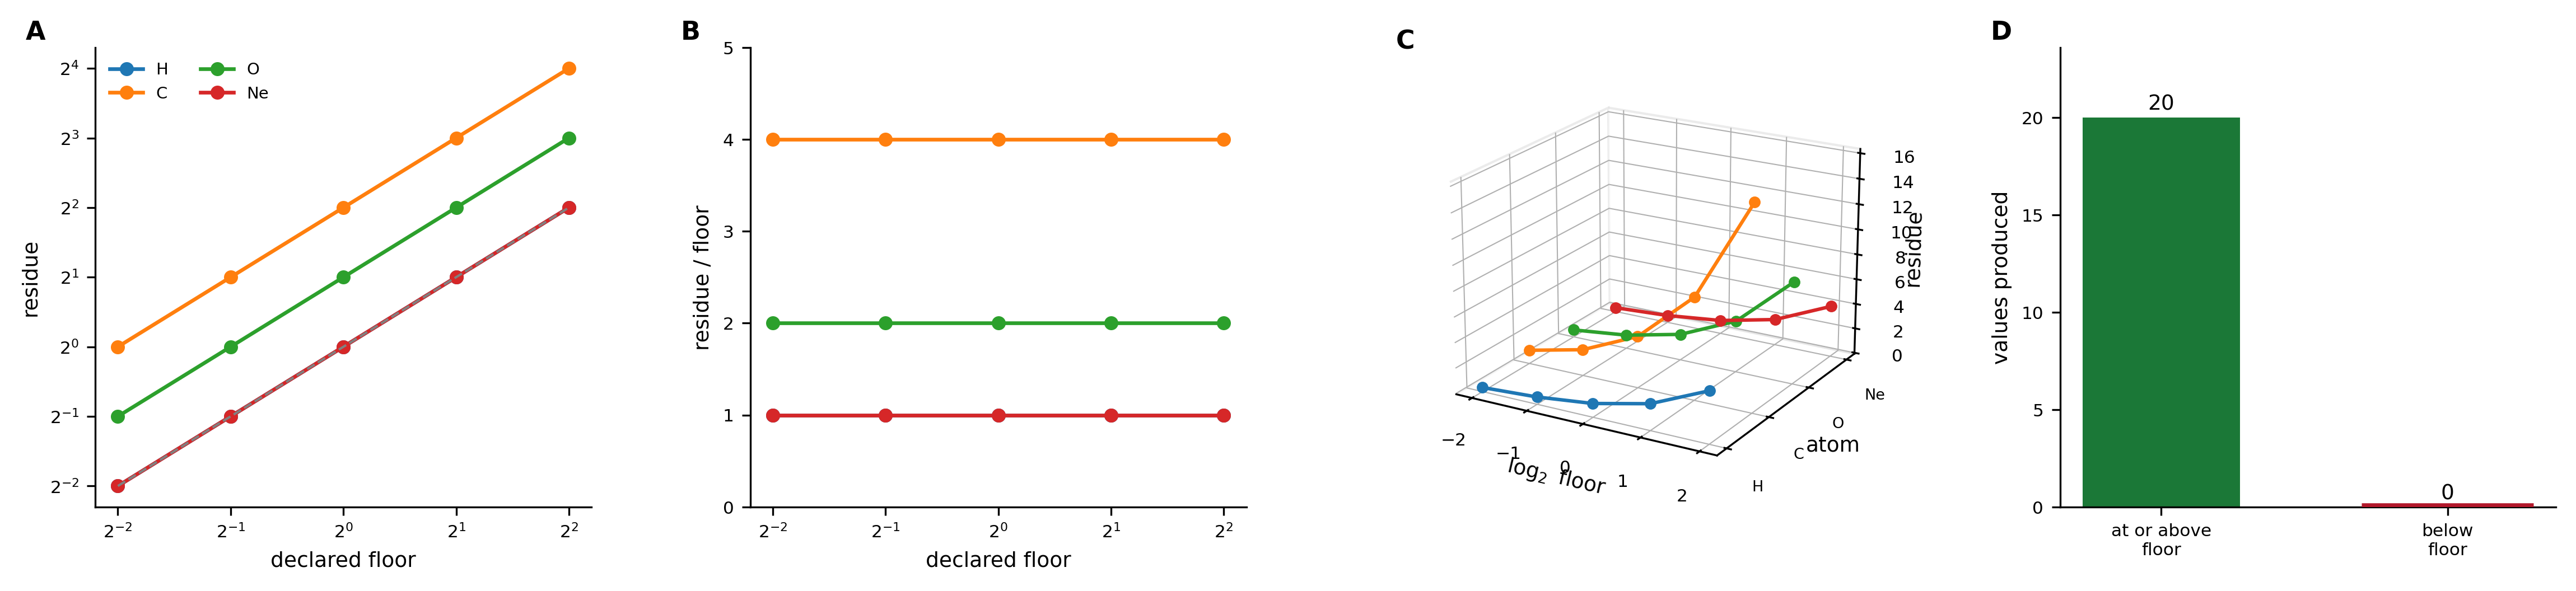
\includegraphics[width=\textwidth]{figures/panel_01_floor.png}
    \caption{\textbf{The floor is a resolution scale the value is
    expressed in, not a truncation applied to a value computed
    independently of it.}
    Conformance item (C1) asks that no program produce a value with
    $\res<\flo$. As \Cref{rem:c1-vacuous} records, that test cannot fail:
    the residue is computed as $\flo\times\nu$ under a $\max(\cdot,\flo)$
    clamp, so a sub-floor value is unconstructible. The informative
    measurement is how the residue \emph{responds} to the floor, which is
    what this panel shows.
    (\textbf{A})~Residue against declared floor on log--log axes for four
    atoms, with the identity dashed. Every trace is a straight line of
    unit slope over a sixteen-fold sweep, $\flo\in\{0.25,\dots,4\}$;
    hydrogen and neon coincide because both have unit multiplier.
    (\textbf{B})~The same data as the ratio $\res/\flo$. Each atom is flat
    across the entire sweep --- $1.0$ for hydrogen, $4.0$ for carbon,
    $2.0$ for oxygen, $1.0$ for neon. Flatness is the claim: a truncation
    applied after the fact would produce a ratio that moved with the
    floor, rising toward $1$ as the floor overtook the value.
    (\textbf{C})~The full sweep in (floor, atom, residue) space. The
    surface is ruled: for fixed atom the residue is linear in the floor,
    and for fixed floor it is a per-atom multiple. Those two facts
    together are what ``the floor is a resolution'' means operationally.
    (\textbf{D})~Values at or above the floor against values below it,
    over all $20$ runs of the sweep. The below-floor count is zero, drawn
    as an explicit floor tick. We report it alongside
    panel~(\textbf{B}) rather than alone, because on its own it is a
    restatement of the clamp rather than evidence about the language.}
    \label{fig:floor}
\end{figure*}

\begin{figure*}[!htbp]
    \centering
    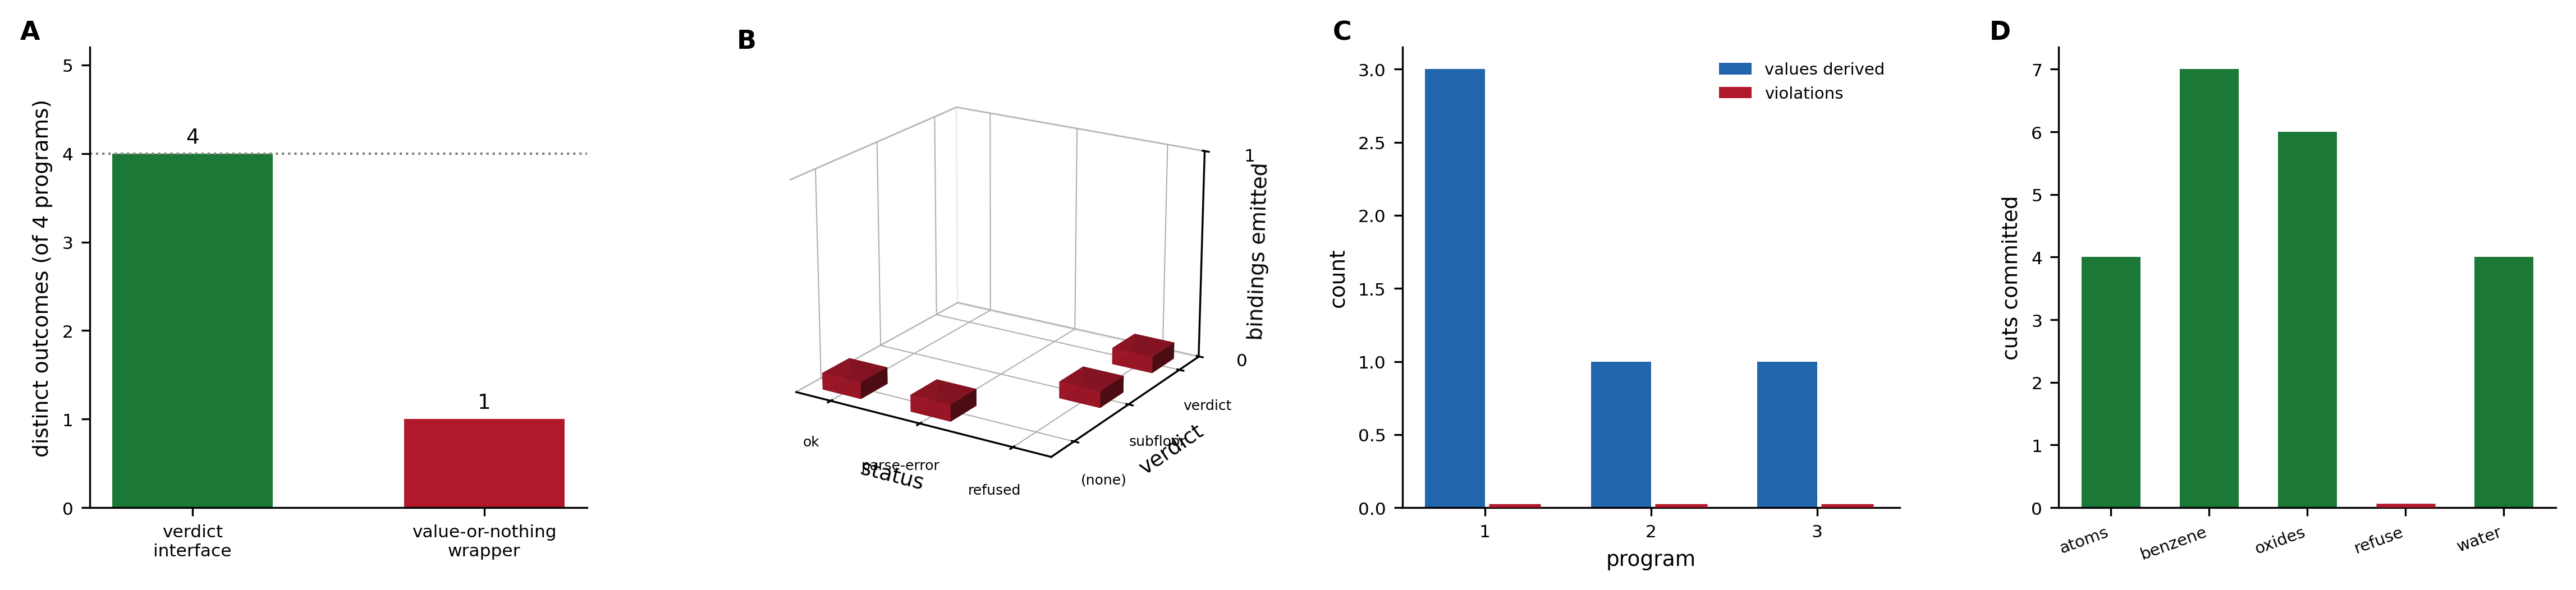
\includegraphics[width=\textwidth]{figures/panel_02_conflation.png}
    \caption{\textbf{Four programs failing for four different reasons are
    four outcomes under the verdict interface and exactly one under a
    value-or-nothing wrapper.}
    The four are a sub-resolution floor, a parse error, an unbound
    reference, and an import refused on provenance.
    \Cref{rem:c4-programs} records why \hj{unclosed} and \hj{inert} are
    not among them: both bind values, so both report \emph{value} under
    the wrapper and would make the control fail for the wrong reason.
    (\textbf{A})~Distinct outcomes under each interface. The verdict
    interface distinguishes all four; the wrapper returns one. That
    collapse is what makes \Cref{thm:conflation} non-vacuous on this
    implementation --- exhibited rather than assumed.
    (\textbf{B})~Each program placed by status and verdict kind, with
    height the number of bindings emitted. All four sit at zero height:
    they occupy four distinct positions in the (status, verdict) plane and
    the same position on the value axis, which is precisely the geometry
    the theorem describes.
    (\textbf{C})~Provenance monotonicity (C2), a separate measured item.
    Values derived per program against violations found. The violation
    count is zero in every program, drawn as explicit floor ticks.
    Composition is maximum, so a $\supplied$ input can never yield a
    $\stated$ output; a violation would be convention laundered into
    record.
    (\textbf{D})~Cuts committed by each example program, coloured by
    whether the program completed. \hj{refuse.hj} commits none, because it
    declines before measuring anything: a refusal costs no cuts, which is
    the operational content of refusing rather than computing and
    discarding.}
    \label{fig:conflation}
\end{figure*}

\begin{figure*}[!htbp]
    \centering
    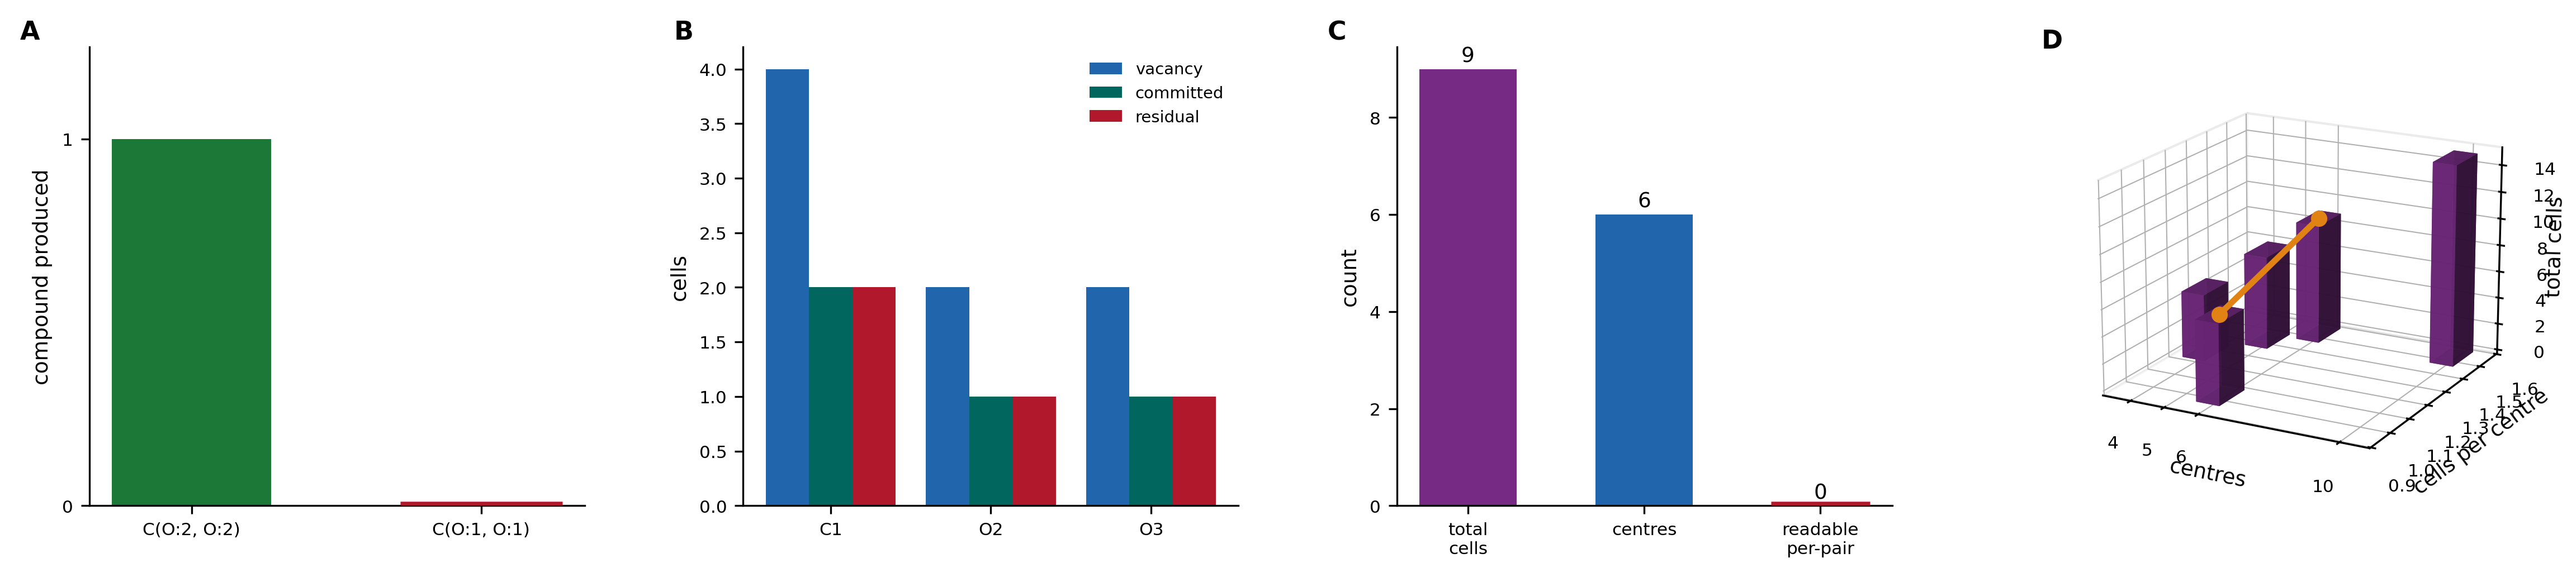
\includegraphics[width=\textwidth]{figures/panel_03_cells.png}
    \caption{\textbf{Committed cell counts change what is built, and a
    delocalised system carries a total that no per-pair count can be
    recovered from.}
    (\textbf{A})~The same atoms at the same stoichiometry under two cell
    commitments. \hj{close C(O : 2, O : 2)} produces a compound;
    \hj{close C(O : 1, O : 1)} produces none, drawn as an explicit zero.
    The difference is stronger than a differing field: one program yields
    a value and the other yields a verdict.
    (\textbf{B})~Why the one-cell reading yields nothing: vacancy,
    committed cells and residual per atom in the \textsf{unclosed}
    verdict. Carbon has vacancy $4$ with $2$ committed, leaving residual
    $2$; each oxygen leaves $1$. A connectivity-only model writes both
    programs as ``carbon bonded to two oxygens'' and cannot express the
    difference, which is conformance item (C5).
    (\textbf{C})~The benzene delocalised system: total cells $9$ over $6$
    centres, and zero readable per-pair values. The implementation names
    a \textsf{per\_pair\_cells} field and holds it null, which we take to
    be the stronger choice --- the absence is declared rather than left
    to be inferred from a missing key. What (C6) forbids is a readable
    count, and none is readable.
    (\textbf{D})~Five delocalised systems the interpreter actually built,
    positioned by centre count and cells per centre, with height the
    total. The orange spine joins the two systems that share a centre
    count of $6$ and carry different totals, $6$ and $9$. Because the
    total is not a function of the centres, it cannot be unpacked into a
    per-pair count by dividing --- which is why (C6) is a claim about the
    value rather than a convention about its presentation.}
    \label{fig:cells}
\end{figure*}

\begin{figure*}[!htbp]
    \centering
    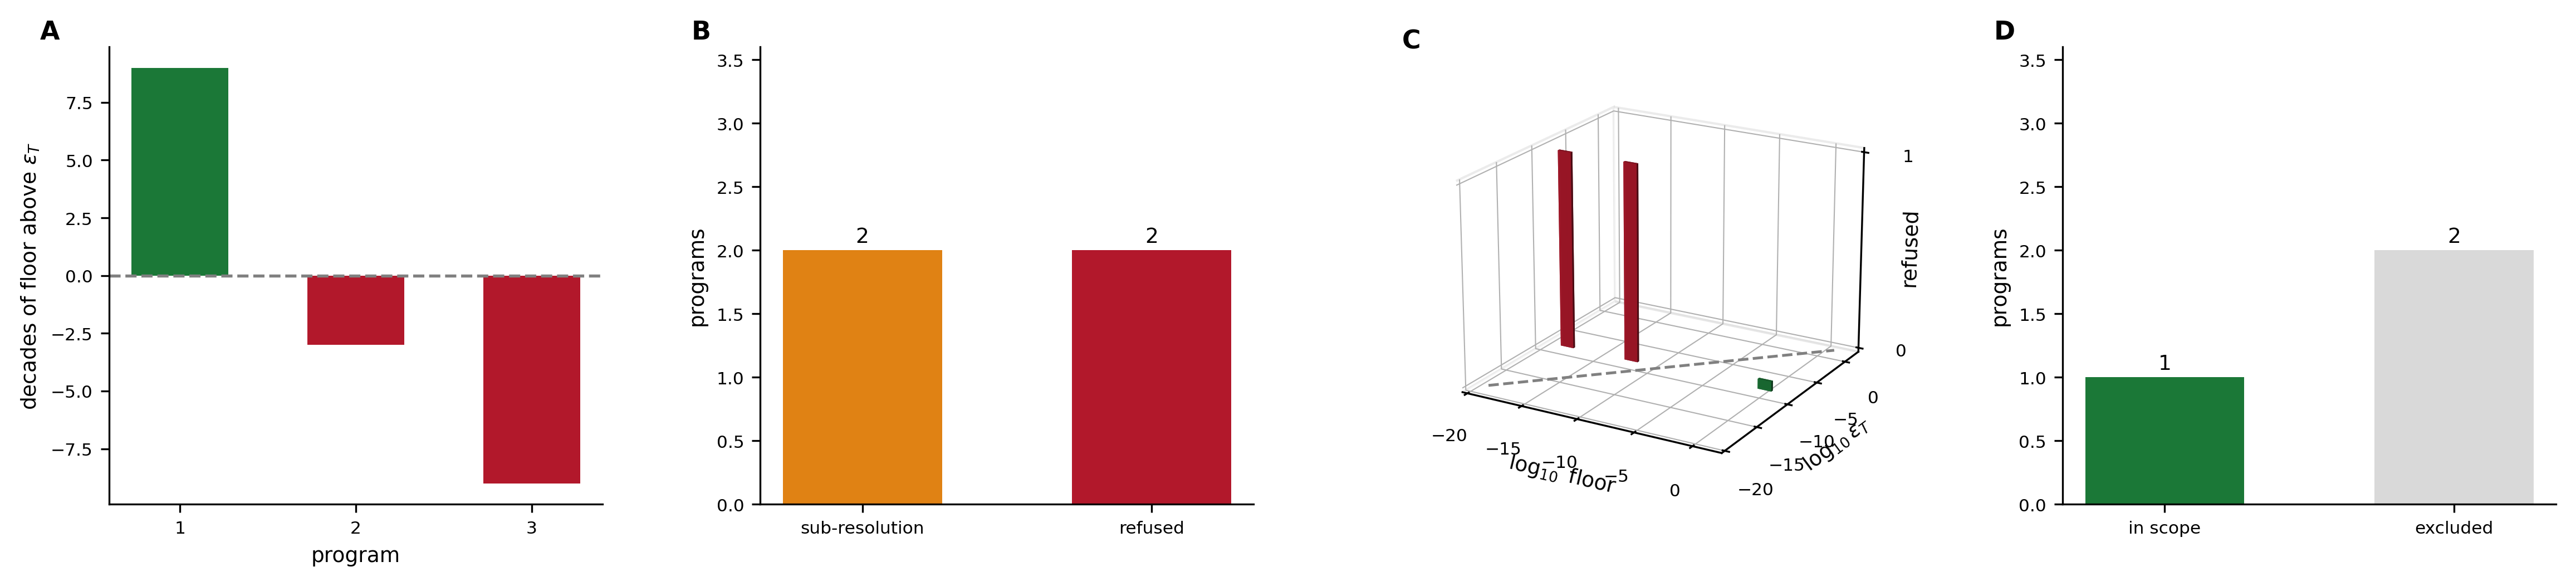
\includegraphics[width=\textwidth]{figures/panel_04_resolution.png}
    \caption{\textbf{A floor finer than the target's resolution is
    refused with both numbers named, and the refused programs are
    excluded from the equivalence claim rather than run and tolerated.}
    (\textbf{A})~Each program's declared floor as decades above the
    target resolution $\eps_T=10^{-9}$, with the gate at zero. One
    program clears it; two fall $3$ and $9$ decades below. The axis is a
    margin rather than a raw $\log_{10}$ floor because the raw quantity
    renders the single admitted program (floor $1.0$, $\log_{10}=0$) as an
    invisible bar while the refused ones become large spikes, which reads
    backwards.
    (\textbf{B})~Programs below the resolution against programs refused.
    The two counts are equal at $2$: the gate fires on exactly the
    programs that trip it, neither over- nor under-refusing.
    (\textbf{C})~The gate in (floor, target resolution, refused) space
    with the line $\flo=\eps_T$ drawn. Bars stand at height $1$ on the
    sub-resolution side and lie flat on the other. The refusal verdict
    carries both numbers, the declared $10^{-12}$ and the target
    $10^{-9}$; \Cref{rem:ambient} notes that the declared value lives in
    the verdict rather than in the interpreter's ambient state, since a
    refused declaration by definition did not take effect.
    (\textbf{D})~Scope of \Cref{thm:target-equiv}: one program in scope,
    two excluded. The in-scope set is a strict subset, which is the
    discipline \Cref{rem:c8} asks for --- a suite that ran the excluded
    programs on both back ends and reported their disagreement as
    tolerable would be asserting the unconditional theorem that
    \Cref{rem:equiv-honest} retracts.}
    \label{fig:resolution}
\end{figure*}


% =====================================================================
\section{What honjo does not do}
\label{sec:limits}
% =====================================================================

\begin{enumerate}[label=\textbf{L\arabic*.},leftmargin=2.8em,itemsep=4pt]

\item \textbf{No bond energetics.} \textsc{Bond} decides whether an
interface lowers boundary thickness and how many cells it commits, not by
how much. honjo therefore cannot rank two candidate structures by
stability, and a program that appears to do so is reading a residue,
which is a separation cost, not an energy
(\Cref{rem:cells-scope}).

\item \textbf{No covalent/ionic distinction.} The underlying operation
treats an interface through vacancy sharing alone, so a bond in which the
shared cells are held very unequally and one in which they are held
evenly are the same object to honjo. This is a limitation of the
chemistry the language binds to, not of the language.

\item \textbf{Multiple bonding is counted, not adjudicated.} The cell
count records how many cells an interface commits. Nothing in honjo
decides \emph{whether} a double interface or two singles is the realised
structure; a program must state which it means. \hj{deloc} is likewise a
declaration, not a perception.

\item \textbf{No file input, no perception.} honjo does not read
records, parse notations, or perceive rings, aromaticity or
stereochemistry. Structures arrive already translated
(\Cref{rem:boundary-scope}).

\item \textbf{Provenance is two-valued and coarse.} The tag distinguishes
stated from supplied and nothing finer: it does not record \emph{which}
convention supplied an element, nor weight elements by importance
(\Cref{rem:max-not-count}). A supplied bond order at a reactive centre
and a supplied aliphatic hydrogen both make a result $\supplied$.

\item \textbf{Soundness is proved as a sketch.} \Cref{thm:soundness} is
argued, not formalised, and the mutation clause is the non-routine step
(\Cref{rem:sketch}). A mechanised proof would be worth having and we have
not carried one out.

\item \textbf{Target equivalence is conditional and the condition is
measured, not derived.} \Cref{thm:target-equiv} holds when
$\eps_R+\eps_T\le\flo$. Whether a given GPU configuration satisfies this
is an empirical property of that hardware which the implementation must
report; the specification requires the check but cannot discharge it
(\Cref{rem:equiv-honest}).

\item \textbf{No performance claim.} Nothing here asserts that the
render-pass realisation is faster than the exact one for any particular
program, only that it is a distinct realisation of the same IR.
\end{enumerate}

% =====================================================================
\section{Conclusion}
\label{sec:conclusion}
% =====================================================================

We have specified Honjo Masamune as a language whose single primitive is
the cut---the act of individuating a part of a bounded whole at the
irreducible cost $\flo>0$---and whose every operation, from generating an
atom to tracking an item through a process, is that primitive at a
different arity.

Three properties are enforced statically. No value may claim zero residue
(\Cref{thm:no-zero-value}), so the sharp cut is untypeable. No operation
may launder supplied data into stated data
(\Cref{thm:prov-monotone,cor:no-launder}), so an audit performed before
honjo survives every computation after it. And no operation that can fail
returns an empty value: it returns a labelled verdict, of which only one
label carries a value (\Cref{prop:one-value}), because a value-or-nothing
interface provably conflates four distinguishable failures that no
caller discipline recovers (\Cref{thm:conflation}).

The surface language gained two forms it previously lacked and needed:
committed-cell counts on bonds, without which multiply-bonded structures
are inexpressible; and a delocalised-system form which is not sugar for
fractional per-bond counts, because \Cref{prop:deloc} shows such counts
state what the system does not. Structures enter through a typed import
that refuses rather than silently accepting a graph whose provenance
falls short of what the program declared it needs.

One earlier claim has been retracted and replaced. Two-target equivalence
was previously asserted unconditionally on the reasoning that a target's
readback error is bounded by the floor; that reasoning conflates a
property of the program's weights with a property of the hardware's
arithmetic. \Cref{thm:target-equiv} now carries the hypothesis
$\eps_R+\eps_T\le\flo$, the implementation must report $\eps_T$, and a
program whose floor is finer than its target can resolve is refused
rather than run (\Cref{cor:refuse-lowfloor}). The conformance suite
records which programs the equivalence covers instead of tolerating
disagreement on the ones it does not.

\Cref{sec:limits} states eight things the language does not do, three of
which are limitations of the chemistry it binds to and cannot repair from
inside. A specification whose worked examples all succeed has not been
shown capable of refusing anything, and refusal is a property this one
claims: \Cref{sec:examples} includes a program that declines to compute,
and \Cref{sec:impl} requires a conformance check that it does.

\bibliographystyle{plainnat}
\bibliography{references}

\end{document}
